\chapter{Exact Algorithms for TSP} \label{chapt:3}

This chapter provides an in-depth examination of exact algorithms for solving the Traveling Salesman Problem (TSP), incorporating detailed pseudo-code to elucidate the operational principles of each method. Through these algorithms, we explore the computational landscape of finding optimal solutions to TSP.

\section{Overview of Exact Algorithms}

Exact algorithms for TSP are characterized by their ability to invariably find the optimal solution, albeit with computational costs that can become prohibitive as the number of cities increases. These algorithms serve as a theoretical and practical foundation for understanding the limits of computationally solving TSP.

\subsection{Brute Force Method}

The brute force method systematically examines every possible tour to identify the one with the lowest total distance. Despite its simplicity, the exponential growth in computations makes it impractical for large instances.

\begin{algorithm}
	\caption{Brute Force TSP}\label{bruteforce}
	\begin{algorithmic}[1]
		\Procedure{BruteForceTSP}{$cities$}
		\State $min\_distance \gets \infty$
		\State $min\_tour \gets \emptyset$
		\ForAll{tours $t$ of $cities$}
		\State $distance \gets$ \textsc{TourDistance}($t$)
		\If{$distance < min\_distance$}
		\State $min\_distance \gets distance$
		\State $min\_tour \gets t$
		\EndIf
		\EndFor
		\State \Return $min\_tour$
		\EndProcedure
	\end{algorithmic}
\end{algorithm}

The computational complexity of this method is $O(n!)$, reflecting the factorial number of tours that must be evaluated.

\subsection{Bellman-Held-Karp Algorithm}

The Bellman-Held-Karp algorithm represents a significant advancement in exact TSP solutions by leveraging dynamic programming to reduce the computational burden. This approach calculates the shortest path by breaking down the problem into smaller subproblems and storing the results of these subproblems to avoid redundant calculations.

\begin{algorithm}
	\caption{Bellman-Held-Karp Algorithm}\label{bellmanheldkarp}
	\begin{algorithmic}[1]
		\Procedure{BellmanHeldKarp}{$cities$}
		\State Create a table $distances$ to store the shortest paths
		\State Initialize all entries in $distances$ to $\infty$
		\State $distances[1][\{1\}] \gets 0$ \Comment{Starting city}
		\For{$m = 2$ to $|cities|$}
		\ForAll{subsets $S$ of $cities$ of size $m$ containing 1}
		\ForAll{$j \in S, j \neq 1$}
		\State $distances[j][S] \gets \min_{k \neq j, k \in S} (distances[k][S\setminus\{j\}] + distance(k, j))$
		\EndFor
		\EndFor
		\EndFor
		\State \Return $\min_{j}(distances[j][cities] + distance(j, 1))$
		\EndProcedure
	\end{algorithmic}
\end{algorithm}

The Bellman-Held-Karp algorithm operates with a time complexity of $O(n^2 \cdot 2^n)$~\ref{fig:agl_complexity}, making it significantly more efficient than the brute force method for moderately sized problem instances. However, the exponential component of its complexity still limits its practical applicability to relatively small TSP instances.

\subsubsection{Branch and Bound}

Branch and Bound is a general algorithmic technique that can be applied to various combinatorial optimization problems, including TSP. It systematically explores the solution space by dividing it into smaller subsets (branching) and using bounds to eliminate subsets that do not contain the optimal solution, thereby reducing the search space.

\begin{algorithm}
	\caption{Branch and Bound for TSP}\label{branchbound}
	\begin{algorithmic}[1]
		\Procedure{BranchAndBoundTSP}{$cities$}
		\State Initialize a priority queue $Q$ with a partial solution starting at the first city
		\State $min\_distance \gets \infty$
		\While{$Q$ is not empty}
		\State Take the partial solution with the lowest bound from $Q$
		\If{it represents a complete tour}
		\If{its cost is less than $min\_distance$}
		\State Update $min\_distance$ and record the tour
		\EndIf
		\Else
		\State Branch by adding a city to the partial solution
		\State Calculate bounds for new partial solutions
		\State Add new partial solutions to $Q$
		\EndIf
		\EndWhile
		\State \Return $min\_distance$
		\EndProcedure
	\end{algorithmic}
\end{algorithm}

The efficiency of Branch and Bound for TSP depends significantly on the bounding function used to estimate the lower bound of partial solutions. Effective bounding can lead to substantial reductions in the search space, allowing the algorithm to find the optimal solution more quickly than exhaustive search methods. However, its worst-case time complexity remains $O(n!)$~\ref{fig:agl_complexity}, which means that for very large problem instances, even this sophisticated approach may not be practical.


\section{Analysis of Exact Algorithms}

\subsection{Computational Feasibility}

Exact algorithms for the TSP, such as the brute force method, dynamic programming, and the Held-Karp algorithm, offer theoretical guarantees for finding the optimal tour. However, their computational feasibility is significantly challenged as the number of cities increases. The factorial growth rate of the brute force method's complexity and the exponential growth rate of dynamic programming and Held-Karp's complexities restrict their practical application to relatively small instances of the TSP.

\begin{center}
	\begin{figure}[h]
		\caption{Exact Algorithms complexity}
		\label{fig:agl_complexity}
		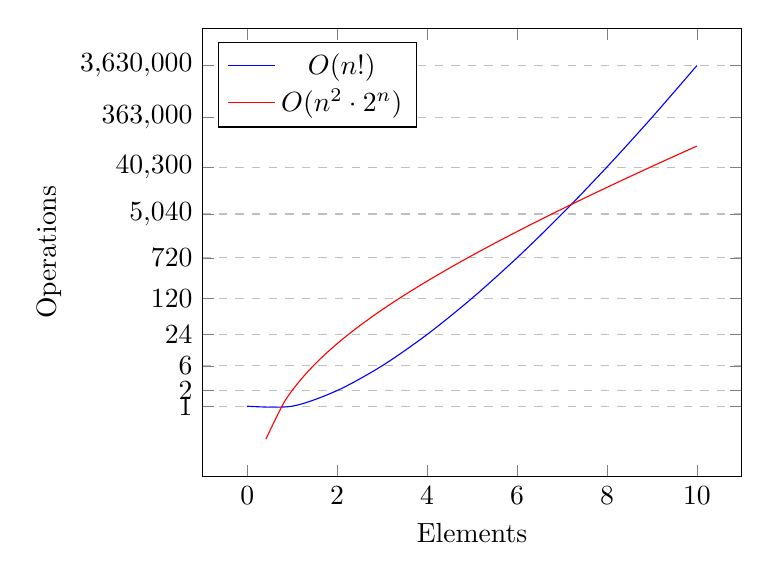
\begin{tikzpicture}
			\begin{semilogyaxis}[
					xlabel={Elements},
					ylabel={Operations},
					domain=0:10,
					ytick={0,1,2,6,24,120,720,5040,40320,362880,3628800},
					log ticks with fixed point,
					legend pos=north west,
					ymajorgrids=true,
					grid style=dashed,
				]
				\addplot+[mark=none,smooth] coordinates {
						(0,1) (1,1) (2,2) (3,6) (4,24) (5,120) (6,720) (7,5040)
						(8,40320) (9,362880) (10,3628800)
					};
				\addlegendentry{$O(n!)$}

				\addplot+[mark=none,smooth] expression {x^2 * 2^x};
				\addlegendentry{$O(n^2 \cdot 2^n)$}

			\end{semilogyaxis}
		\end{tikzpicture}
	\end{figure}
\end{center}

\subsection{Pros and Cons}

\textbf{Pros:}
\begin{itemize}
	\item Guarantee of finding an optimal solution.
	\item Provide a benchmark for evaluating the performance of heuristic and metaheuristic algorithms.
\end{itemize}

\textbf{Cons:}
\begin{itemize}
	\item Exponential time complexity makes them impractical for large instances.
	\item Significant computational resources required for even moderate-sized problems.
	\item Dynamic programming and Held-Karp, while more efficient than brute force, still face limitations due to their space complexity and the need for extensive computation.
\end{itemize}

The exploration of exact algorithms lays the foundation for understanding the computational intricacies of the TSP. While their practical application is limited by their computational demands, they remain crucial for theoretical analysis and for setting the stage for alternative solving techniques discussed in subsequent chapters.
